%   Filename    : chapter_4.tex 
\chapter{Methodology}
This chapter outlines the systematic approach that were taken to address the problem of pothole depth estimation using StereoPi V2. The methodology is divided into key phases: data collection, algorithm selection, design, testing and experimentation, and challenges and limitations. Each phase will play a crucial role in accurately classifying and assessing road defects.  Each phase is essential for accurately estimating the depth of potholes using StereoPi V2. 

\section{ Research Activities}

\subsection{Data Collection}
The researchers conducted initial inquiries to understand the problem domain and existing road maintenance practices. This phase included consulting the engineers under the Road Maintenance Department of the government agency Department of Public Works and Highways (DPWH). An interview with Engr. Jane Chua provided a comprehensive overview of the DPWH's road maintenance manual, which was crucial in aligning this project with existing standards. This collaboration with DPWH provided insights into road pothole classification standards, ensuring that the collected data will align with industry standards. The DPWH manual primarily focuses on the volume of detected potholes within a road segment as a measure of severity. However, since depth is not explicitly measured in their current procedures, the study will supplement this by referencing international standards such as the Long-Term Pavement Performance (LTPP) classification used in the United States (Miller et al., 2014). The LTPP categorizes potholes based on depth thresholds, which will be integrated with DPWH’s volume-based assessment to provide a more comprehensive severity classification framework. The data collection involved capturing around 130 images of potholes from various locations within the UP Visayas Campus. Ground truth data of pothole depth were collected by the researchers by measuring the depth of different points in an individual pothole and then solving for its average depth. The aforementioned process was validated by Engr. Benjamin Javellana, Assistant Director of the DPWH Regional Office 6 Maintenance Division. In order to individually locate or determine each pothole where the ground truth data is collected, images taken were labeled with their corresponding coordinates, street names, and nearby landmarks.

\subsubsection{Data Collection (Ground Truth Data)}
Data collection took place between January and March 2025, during which the researchers collected depth information from 130 potholes around the University of the Philippines Visayas Miagao Campus. During data collection, the researchers are equipped with safety vests and an early warning device to give caution to incoming vehicles. To measure the depth of each pothole, the researchers recorded four depth points within the pothole and calculated their average.

%\subsection{Algorithm Selection} 
%Potential solutions, algorithms, and system architectures were discussed by the researchers and the special problem adviser in this phase. These sessions, conducted in class and virtually via Zoom, helped narrow down the overview of the system, leading to the selection of the main architecture Epipolar Spatio-Temporal Networks (ESTN) for depth estimation. 

%\subsubsection{Pothole Detection}
%YOLOv5 was selected due to its high accuracy and ability to process images in real-time, making it suitable for detecting road defects in dynamic environments. Its architecture is optimized for speed and performance, which is crucial for large-scale deployment in road inspections. 

%\subsubsection{Severity Assessment}
%The Multi-view Depth Estimation using Epipolar Spatio-Temporal Networks was selected due to the high cost and limited accessibility of LiDAR technology. By applying epipolar geometry and temporal consistency across sequential frames, this approach provides an accurate depth estimation from standard video footage \cite{long2021}. 

\subsection{Design, Testing, and Experimentation}
This section outlines both the design and testing of the system, as well as the experimentation process to validate the selected methodologies. 

\subsubsection{Depth Measurement}
Depth estimation is performed by generating disparity maps from the calibrated stereo image pairs captured by the StereoPi V2. In this process, two key measurement points are selected for each pothole: one targeting the pothole area itself, and another targeting the adjacent road surface considered as the reference plane. By calculating the difference in disparity values between these two points, the system estimates the relative depth of the pothole. This approach improves accuracy by normalizing disparity measurements against the nearby road surface, effectively isolating the pothole’s depth from overall scene variation.

The disparity-to-depth conversion utilizes an inverse model derived from calibration data, ensuring that the depth estimates reflect real-world distances accurately within the effective operational range of the stereo camera setup.

\subsubsection{Severity Assessment}

The estimated pothole depths were classified using the Long-Term Pavement Performance (LTPP) depth thresholds, an internationally recognized framework for pavement distress evaluation. This classification provides standardized criteria to assess pothole severity objectively based on measured depth values. Specifically, potholes with depths less than 2.5 cm are categorized as low severity, those between 2.5 cm and 5 cm as medium severity, and potholes exceeding 5 cm are classified as high severity (Miller et al., 2014)


%\subsubsection{Model Design}
%The system was designed to operate with two core components: YOLOv5 for pothole detection and ESTN for depth estimation. The model architecture was chosen based on the real-time processing capabilities and the need for accurate depth estimation from standard video footage. The design ensures that the system can detect defects and provide severity assessments in a seamless workflow. 

%\subsubsection{Data Set}
%The YOLOv5 model was trained using two datasets from Universe Roboflow. One of the data sets was posted by a user named Eric Tam. It was also stated that the images from the dataset are sourced from a Crowdensing-based Road Damage Detection Challenge from 2022 in Japan. The challenge involves contestants being required to submit road damage datasets, shortlist their data set, and use the data set for road damage detection and classification models. The use of this data set in training models for road damage detection and classification ensures that the data is viable for training the YOLOv5 model. The dataset contains various road defects in Japan.
%Another data set used in training the YOLOv5 model was also uploaded in Universe Roboflow by a user named Atikur Rahman Chitholian which was stated to be part of his undergraduate thesis. The dataset is comprised of 665 images with potholes being labeled. It was also stated that the data set can be utilized in automatically detecting and categorizing potholes found in the streets of cities.
%Data preprocessing techniques were applied to both datasets to improve model accuracy and generalization. These included resizing images to a uniform size, applying %augmentation techniques (flipping, rotation, and color adjustment) to increase dataset variability, and normalizing pixel values to ensure consistency across images. 
\subsubsection{Materials and Equipment}


The prototype system was constructed using several hardware components, which include the items listed below and shown in Figure 3.1:
\begin{itemize}
	\item StereoPi V2 Board
	\item Raspberry Pi Compute Module 4 (CM4)
	\item Dual RaspberryPi Camera Modules with Fisheye Lens
	\item 3D Printed Custom Housing
	\item 2-inch LCD Module
	\item Micro SD Card
	\item Antenna
	\item Momentary Push Button
\end{itemize}

%Parts picture%
\begin{center}
	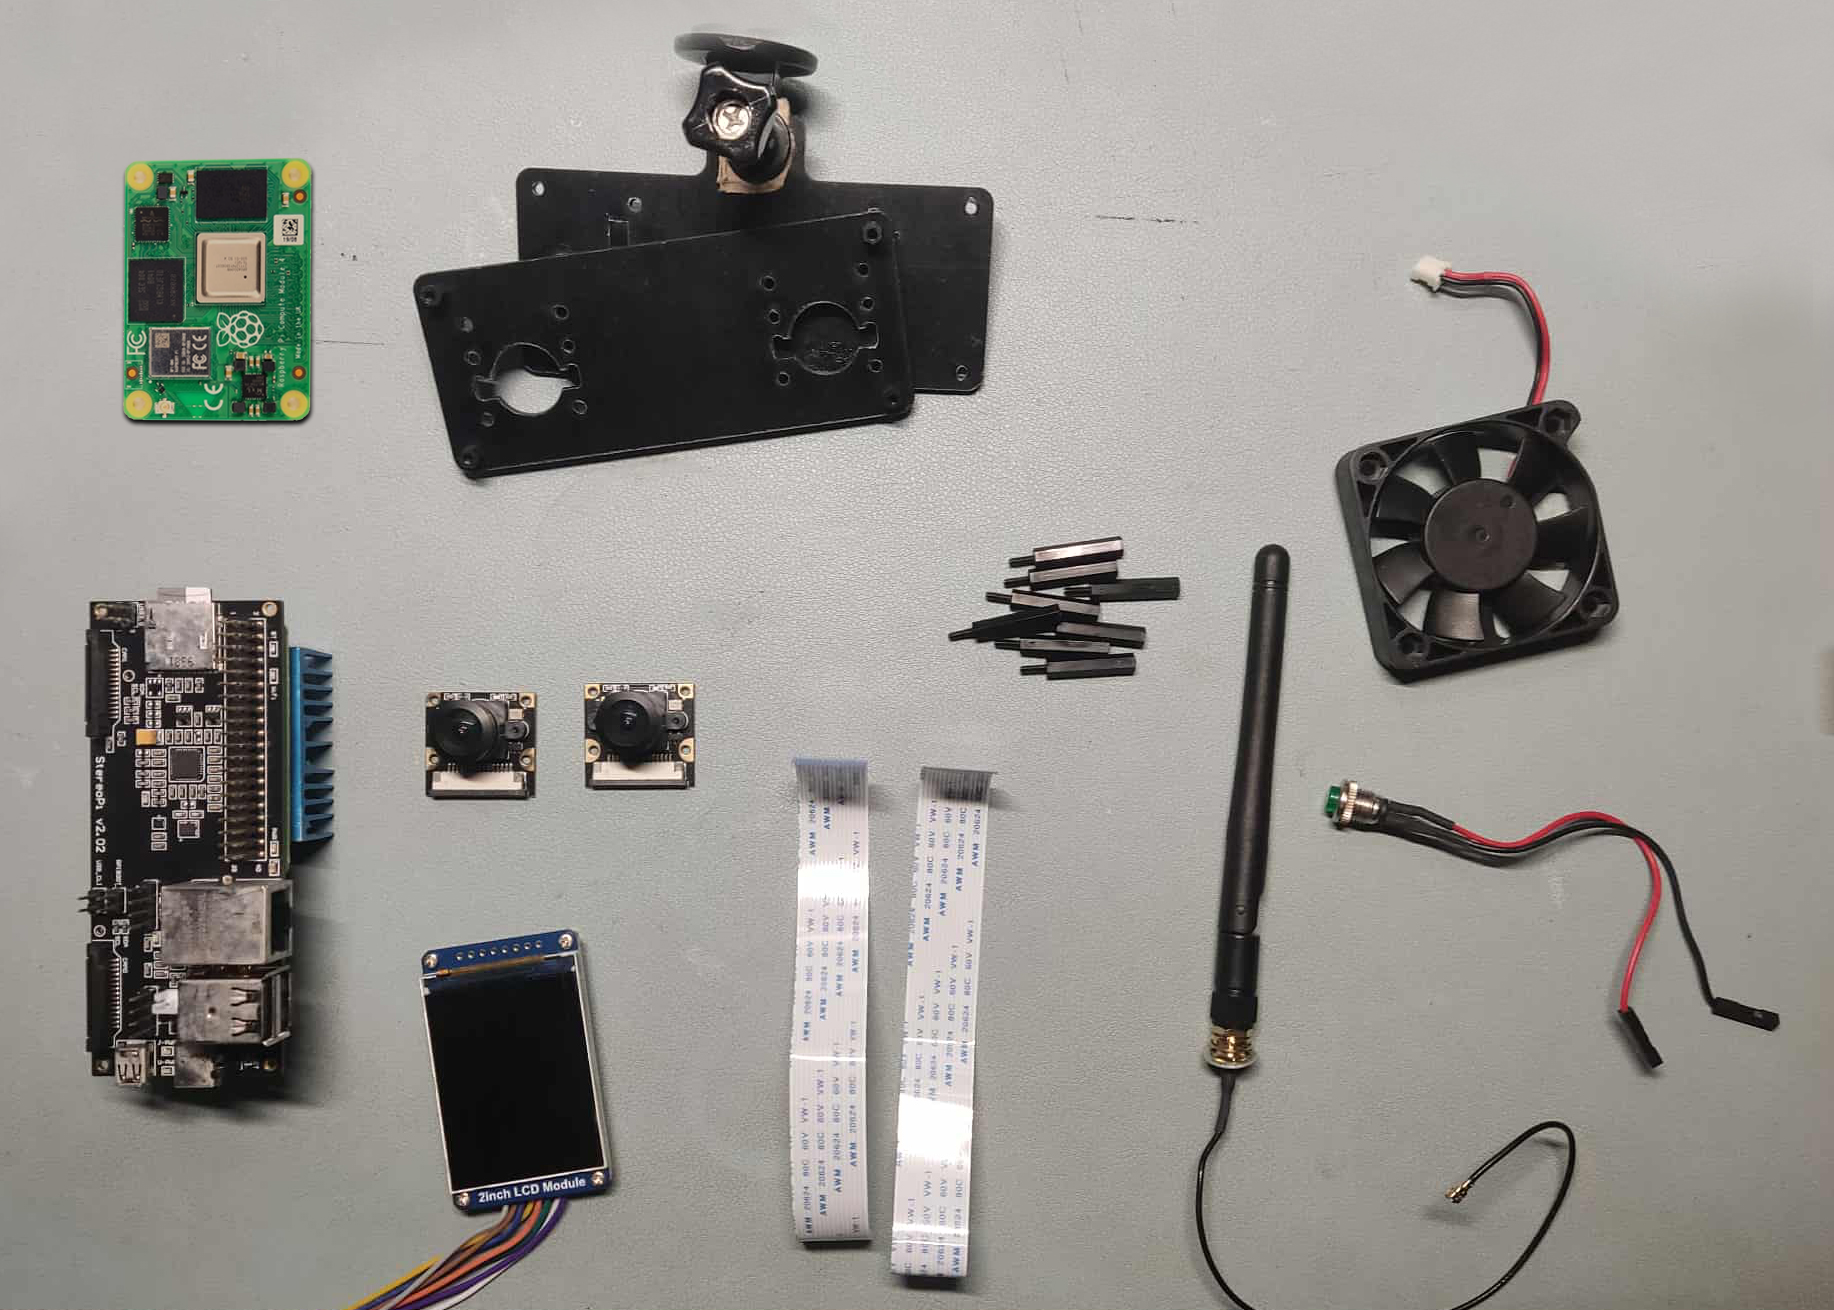
\includegraphics[width=\textwidth]{Parts.png}
	\captionof{figure}{Components used in the prototype development.}
\end{center}



\subsubsection{Prototype Building}
The prototype involved the StereoPi V2 Kit which was acquired through an official international distributer. After assembling the camera, it was further modified to address the it's heating by incorporating a heat sink and a small computer fan to make it suitable for outdoor use.


\begin{minipage}{0.45\textwidth}
	\centering
	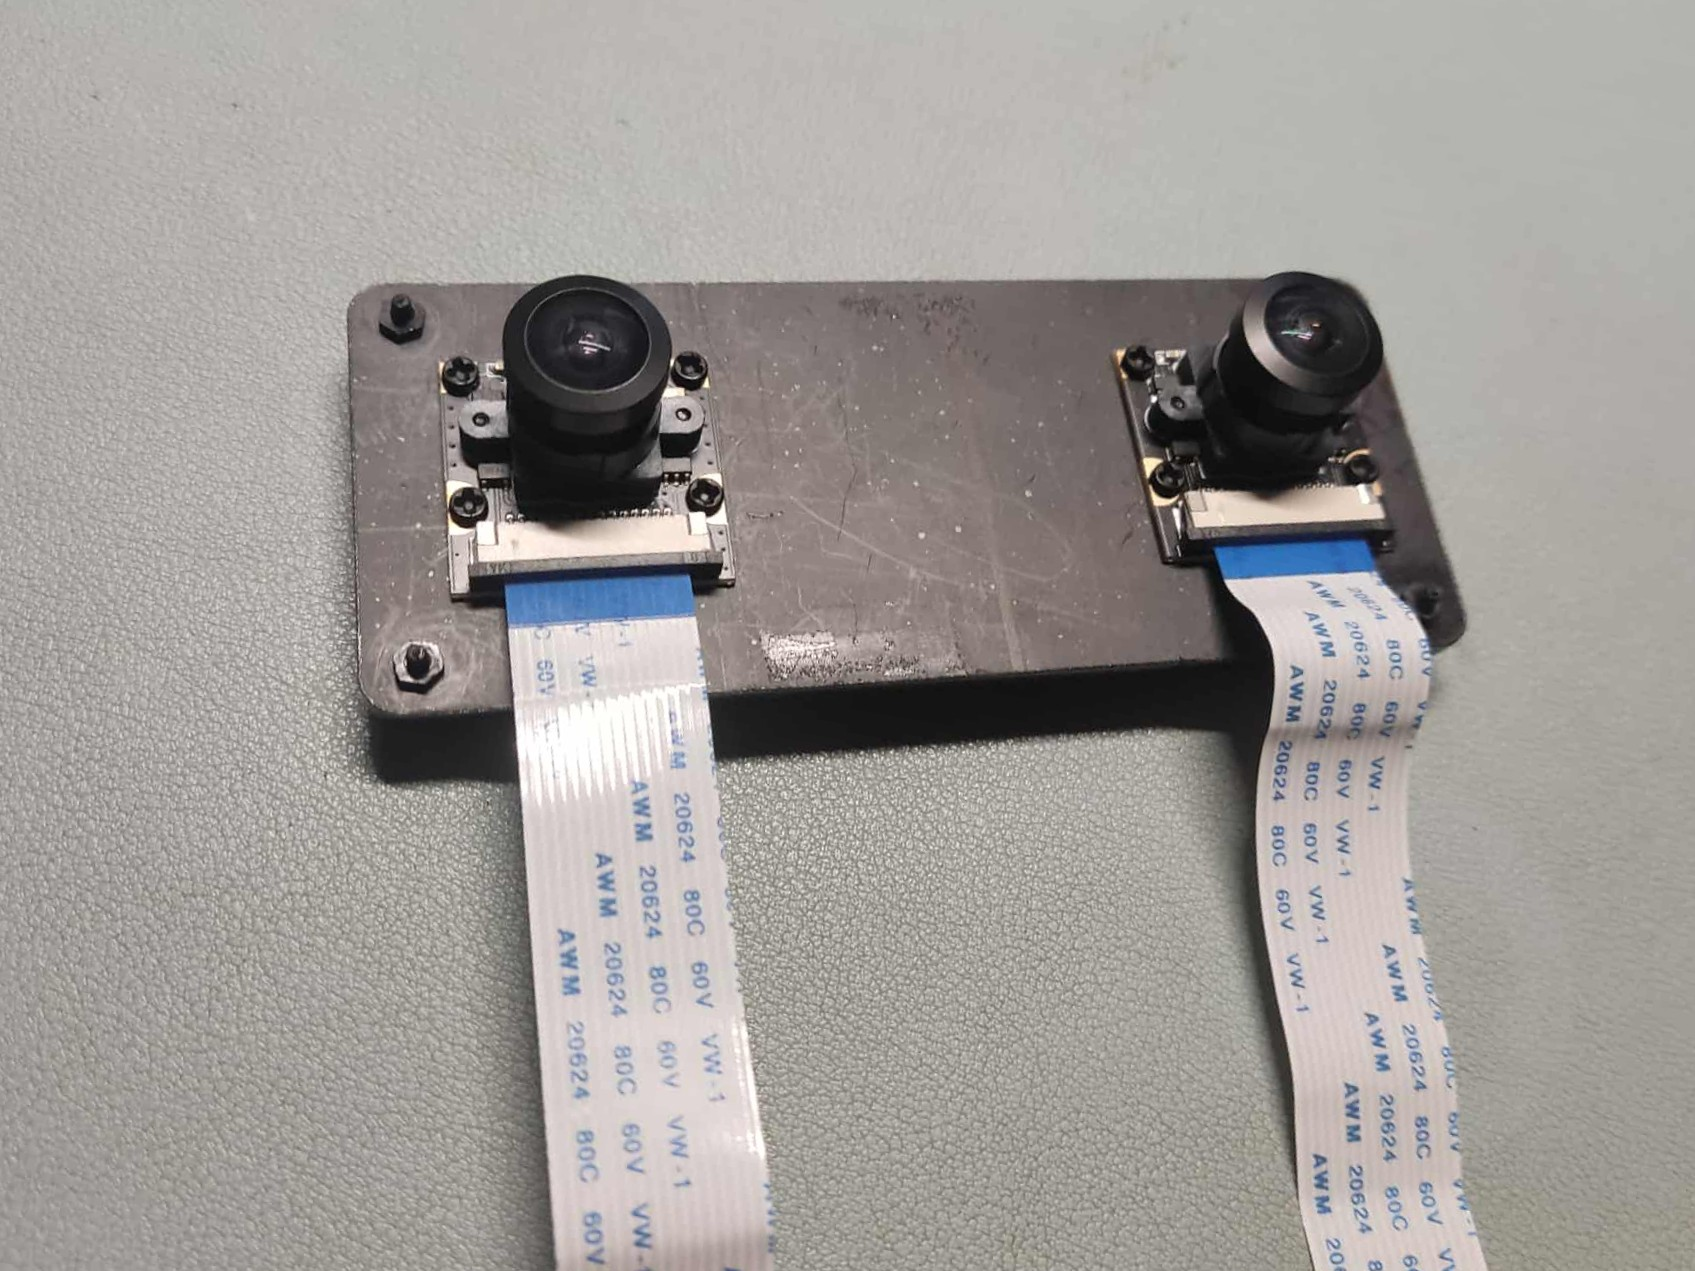
\includegraphics[width=\textwidth]{3.jpg}
	\captionof{figure}{Dual RPi Camera Modules attached to the custom housing.}
\end{minipage}
\hfill
\begin{minipage}{0.45\textwidth}
	\centering
	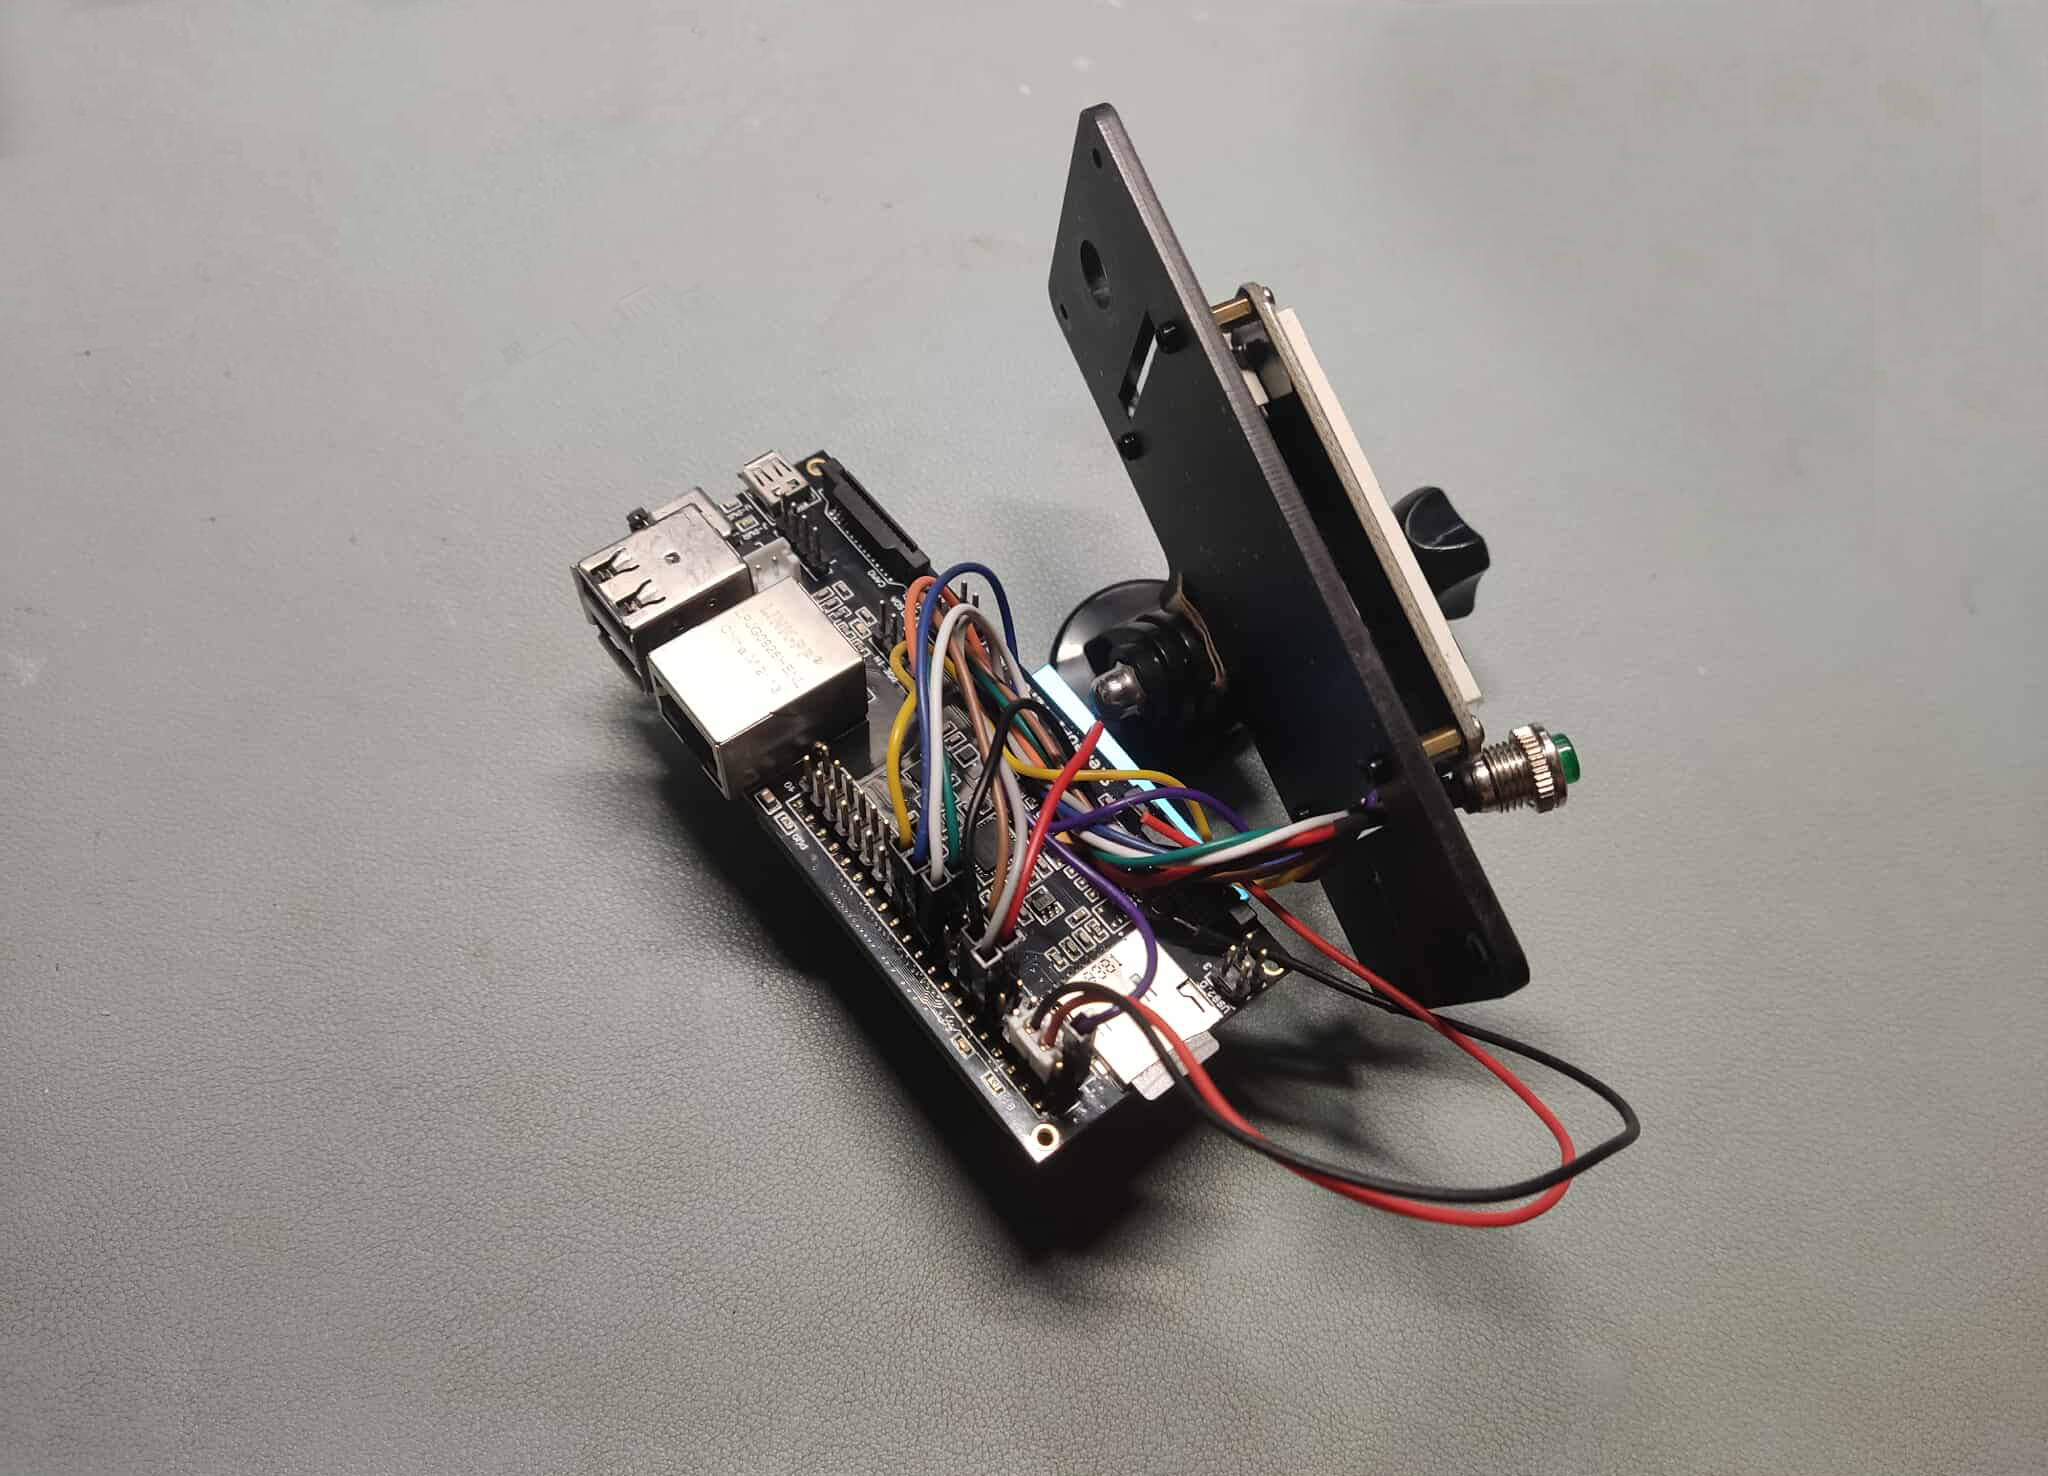
\includegraphics[width=\textwidth]{1.jpg}
	\captionof{figure}{LCD Module connected to the StereoPi board.}
	\label{fig:pic2}
\end{minipage}

%Partial Build%
\begin{center}
	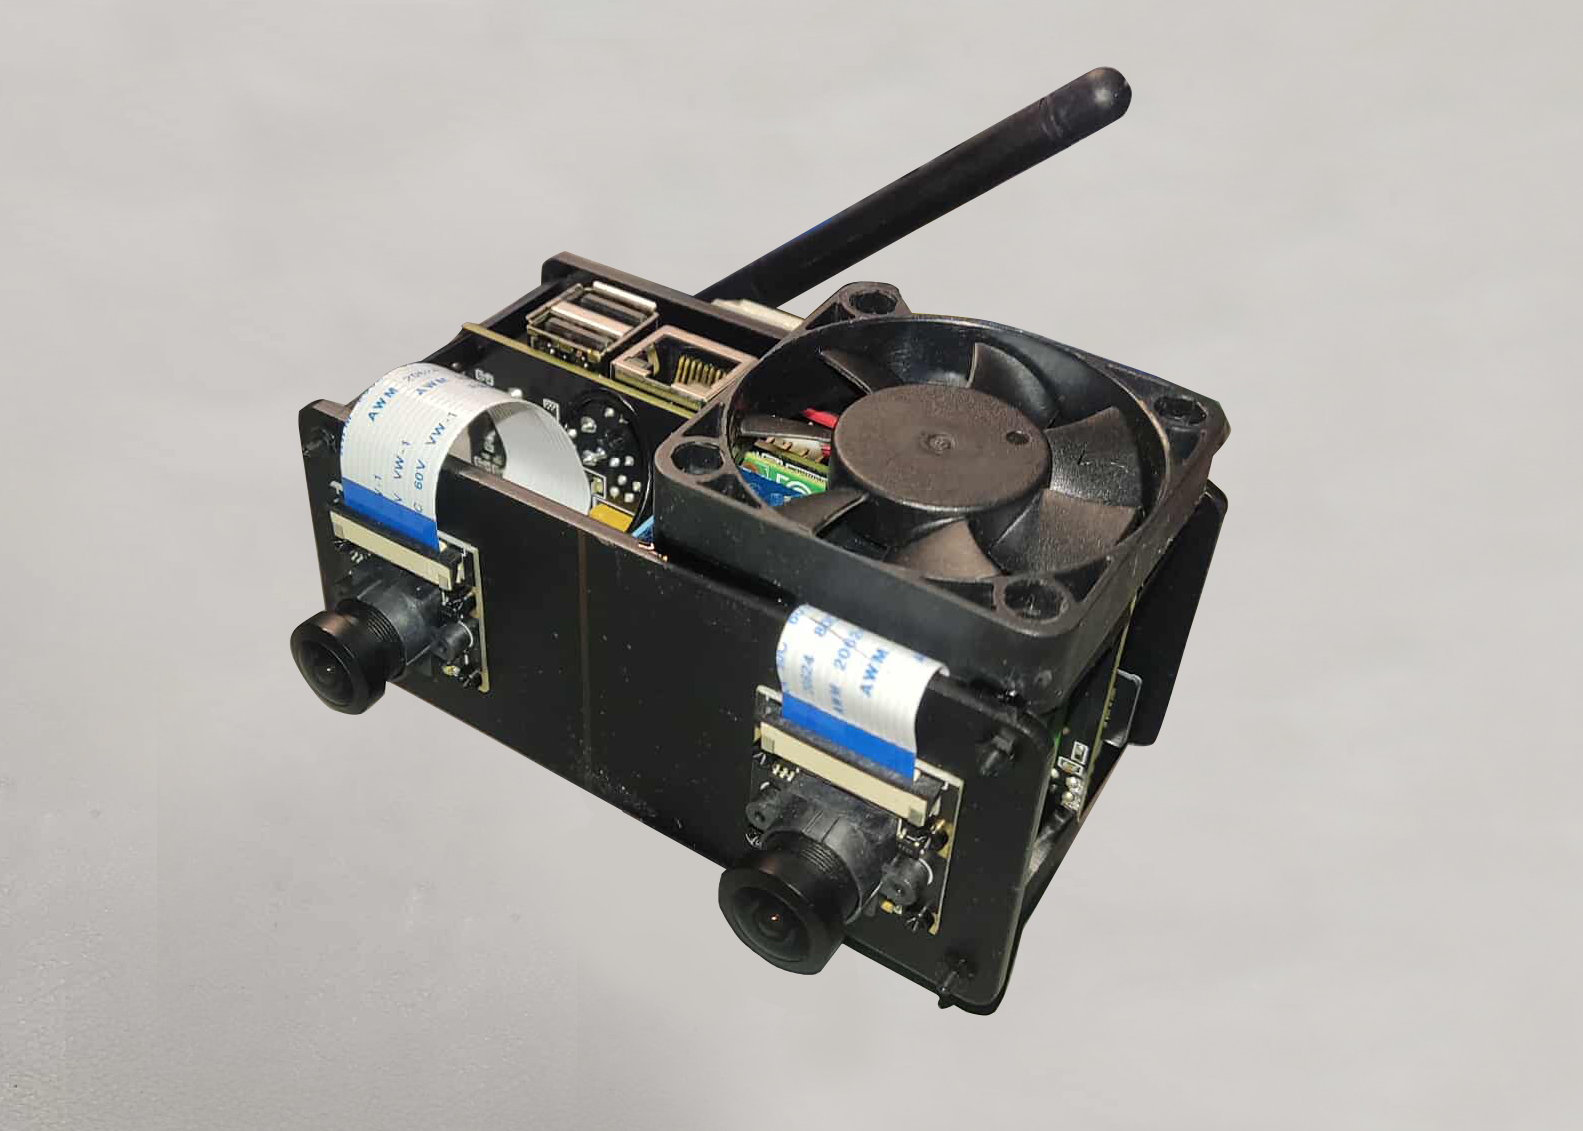
\includegraphics[scale=0.20]{prototype.png}
	\captionof{figure}{The finished prototype.}
\end{center}


\subsubsection{Camera Calibration (Fisheye Distortion)}
The StereoPi V2 is first calibrated using a 9 by 6 checkerboard, with a checker size of 55mm, from different angles through calibration scripts that came with the package. This process ensured that the camera is working properly in capturing stereo imagery. This removed distortion from captured images allowing depth estimation with more accuracy. 

%calibration
\begin{center}
	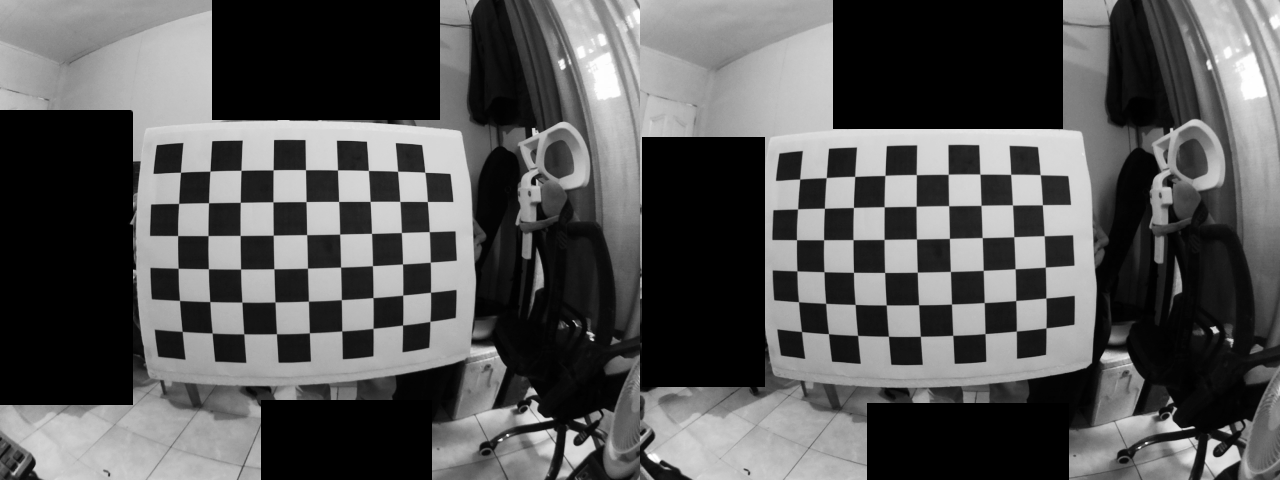
\includegraphics[scale=0.25]{calibration.png}
	\captionof{figure}{Calibration process with a checkerboard to correct fisheye lens distortion.}
\end{center}

\subsubsection{Camera Calibration (Disparity  Map Fine-tuning)}
The stereo image pairs captured by the system were first rectified to ensure proper alignment of corresponding features. Block matching parameters were then fine-tuned to produce clearer and more accurate disparity maps. It was observed that the effective operational range of the stereo camera system extends from approximately 30 to 80 cm. At distances closer than 30 cm, the disparity maps exhibited significant noise, while at distances beyond 80 cm, disparity information became sparse or blank.

%calibration2
\begin{center}
	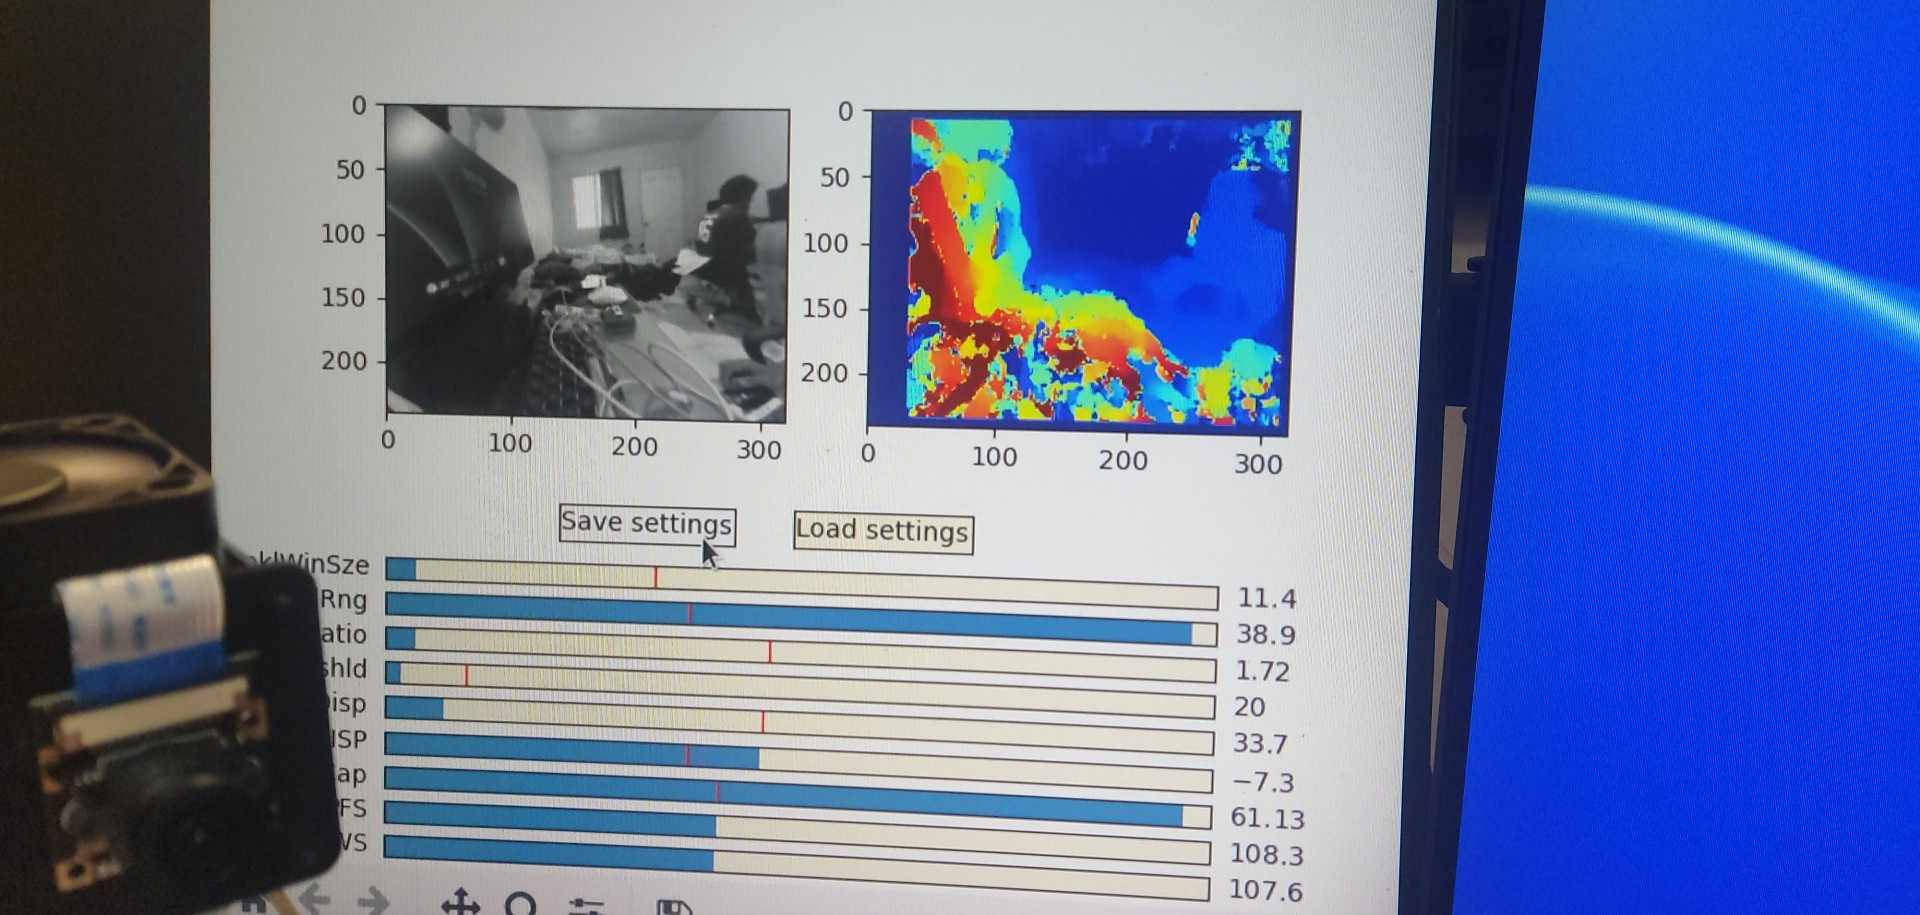
\includegraphics[scale=0.15]{calibration2.jpg}
	\captionof{figure}{Parameter tuning process to achieve cleaner and more accurate disparity maps.}
\end{center}

\subsubsection{Initial Testing}
Initial testing was conducted to verify the functionality and basic accuracy of the stereoscopic camera system in a controlled environment. Artificial potholes with known depths were created to simulate varying real-world scenarios. The system captured disparity maps, and estimated depths were computed using the standard stereo camera depth formula.

%initial test
\begin{center}
	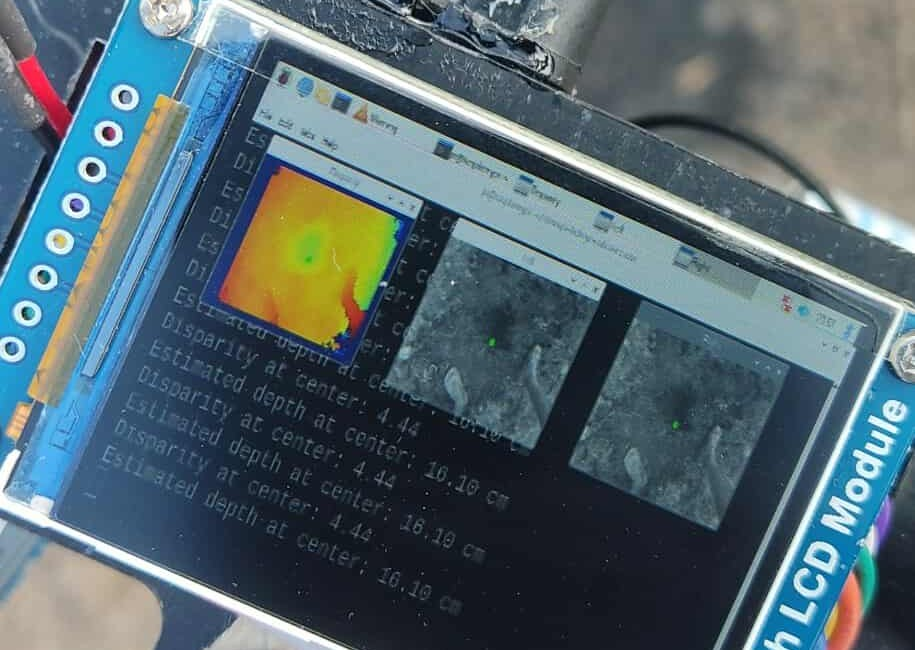
\includegraphics[scale=0.35]{initialtest.jpg}
	\captionof{figure}{The system tested on a simulated pothole.}
\end{center}

However, the results revealed a non-linear relationship between the computed disparity values and the actual distances. This discrepancy indicated that the traditional depth estimation method was insufficient for the current setup. To address this, the researchers collected multiple data points and correlating known distances to their respective disparity readings and fitted an inverse model to better represent the system's behavior (see Figure \ref{fig:model}). This updated disparity-to-depth model was subsequently used in the final testing phase.

%initial test
\begin{figure}[H]
	\centering
	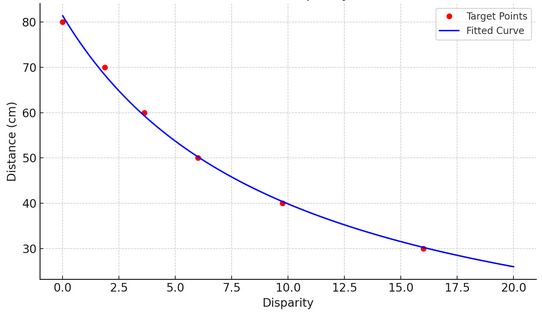
\includegraphics[scale=0.55]{inversemodel.png}
	\caption{Inverse Model Fit to Disparity vs. Distance.\\}
	\label{fig:model}
\end{figure}




\subsubsection{Performance Metrics}
The accuracy of the pothole depth estimated by StereoPi V2 was analyzed using Linear Regression in order to model the difference between the disparity and distance. The lower the disparity indicates that the pothole is deeper.

%The performance of the YOLOv5 model will be evaluated using mean Average Precision (mAP). mAP is a widely used metric in object detection tasks and is particularly useful for assessing models that need to detect and classify multiple object categories. In this case, mAP will provide a comprehensive evaluation of the model's ability to detect and classify potholes, offering an aggregated score across the relevant detection thresholds. This ensures a balanced assessment of both detection accuracy and classification performance, which is essential for accurately identifying potholes across varying conditions. The effectiveness of mAP for this task is well-established in object detection literature (Everingham et al., 2015; Lin et al., 2014).



%For the accuracy of depth estimation using the Epipolar Spatio-Temporal Networks (ESTN), Root Mean Squared Error (RMSE) and Mean Absolute Error (MAE) will be used. RMSE is chosen for its ability to penalize larger errors more heavily, making it suitable for assessing depth estimation performance where larger deviations from the ground truth are more significant (Zhang et al., 2018). MAE is also employed to provide a straightforward measure of average error magnitude, offering a complementary evaluation of depth estimation without emphasizing larger errors as much (Zhang et al., 2020).

\subsubsection{Final Testing and Validation}
The testing process began with a detailed testing plan that includes both simulated and real-world testing scenarios. Initially, the system is tested in controlled environments to ensure it can estimate pothole depth effectively. Following this, real-world testing was conducted using the StereoPi kit on previously located potholes, specifically at the University of the Philippines Visayas Miagao Campus. The system's performance was validated by comparing its predictions with ground-truth data collected from manual inspections. 

\subsubsection{Documentation}
Throughout the research activities, thorough documentation was maintained. This documentation captured all methods, results, challenges, and adjustments made during the experimentation phases. It ensured the reproducibility of the work and provided transparency for future research endeavors. 

\subsection{Challenges and Limitations}

\subsubsection{Camera Limitations}
During the data collection process, the researchers were faced with various issues involving the StereoPi V2 kit. Issues like inaccuracies in the rectified image pair and generated disparity map were very apparent in the early stages of data collection due to limited related studies and literature involving the camera. In addition, the camera also yielded some inaccurate depth estimation and over reliance on controlled environments which prompted the researchers to further improve its tuning and calibration.

%\subsubsection{Availability of Local Datasets}
%The lack of locally labeled datasets for road defects has posed a challenge in training accurate models. The majority of available datasets are sourced from international locations, which may not fully represent the road conditions found in the study area. To address the lack of locally labeled datasets, the researchers will create a pilot dataset from local roads within the University of the Philippines Visayas Miagao Campus. This dataset will be manually annotated according to DPWH's classification standards, ensuring local relevance.

%\subsubsection{Data Quality and Variability}
%Variations in the quality and resolution of the data collected from different sources may impact the performance of the trained models. In particular, images captured under varying weather conditions or lighting may affect the accuracy of pothole detection. To address this, the researchers plan to use the StereoPi kit to capture images under optimal weather and lighting conditions, such as mid-morning or early afternoon on clear days, ensuring consistent image quality for stereo vision analysis. The kit’s stereo cameras will be calibrated for uniform resolution and focus. Data augmentation techniques will also be applied to simulate varying conditions, and pre-processing steps like noise reduction and contrast enhancement will be used to improve the quality of the captured data. This approach aims to minimize the impact of environmental factors on the accuracy of road pothole detection and depth estimation.


%\section{Calendar of Activities}
%Table 1 shows a Gantt chart of the activities. Each bullet represents approximately one week's worth of activity.
%
%  the following commands will be used for filling up the bullets in the Gantt chart
%
%\newcommand{\weekone}{\textbullet}
%\newcommand{\weektwo}{\textbullet \textbullet}
%\newcommand{\weekthree}{\textbullet \textbullet \textbullet}
%\newcommand{\weekfour}{\textbullet \textbullet \textbullet \textbullet}

%
%  alternative to bullet is a star 
%
%\begin{comment}
   %\newcommand{\weekone}{$\star$}
  % \newcommand{\weektwo}{$\star \star$}
  % \newcommand{\weekthree}{$\star \star \star$}
  % \newcommand{\weekfour}{$\star \star \star \star$ }
%\end{comment}



%\begin{table}[ht]   %t means place on top, replace with b if you want to place at the bottom
%\centering
%\caption{Timetable of Activities for 2024} \vspace{0.25em}
%\begin{tabular}{|p{2in}|c|c|c|c|c|} \hline
%\centering Activities (2024) & Aug   & Sept & Oct & Nov & Dec  \\ \hline
%Pre-proposal Preparation      &  \weekfour     &     &  &  &   \\ \hline
%Literature Review & ~~~\weekthree  & \weekone  & &  &    \\ \hline
%Data Collection     &  \weektwo & \weektwo  &  &  &  \\ \hline
%Algorithm Selection     &   & \weektwo &  &  &  \\ \hline
%System Design      &   & \weekone  & \weektwo & ~~~\weektwo &    \\ \hline
%Preliminary Testing &   &  &  & \weektwo & \weekone  \\ \hline
%Documentation and SP Writing & ~~~\weekfour & \weekfour & \weekfour & \weekfour & \weektwo \\ \hline
%\end{tabular}
%\label{tab:timetableactivities}
%\end{table}

%\begin{table}[ht]   %t means place on top, replace with b if you want to place at the bottom
%	\centering
%	\caption{Timetable of Activities for 2025} \vspace{0.25em}
%	\begin{tabular}{|p{2in}|c|c|c|c|c|c|} \hline
%		\centering Activities (2025) & Jan   & Feb & Mar & Apr & May & Jun  \\ \hline
%		Data Collection      &  \weekfour     &     &  &  & &  \\ \hline
%		System Design & ~~~\weekthree  & \weektwo  & \weektwo &  & &   \\ \hline
%		Model testing     &  \weekthree & \weekfour  &  \weekfour &  &  & \\ \hline
%		Results Analysis    &   &  &  \weektwo & \weekfour& & \\ \hline
%		Conclusion Formulation     &   &   &  & ~~~\weektwo &  ~~~\weekthree &  \\ \hline
%		Documentation and SP Writing & ~~~\weekfour & \weekfour & \weekfour & \weekfour & \weekfour &% \weektwo\\ \hline
%	\end{tabular}
%	\label{tab:timetableactivities}
%\end{table}


